\begin{frame}
\frametitle{Mining hospital data}
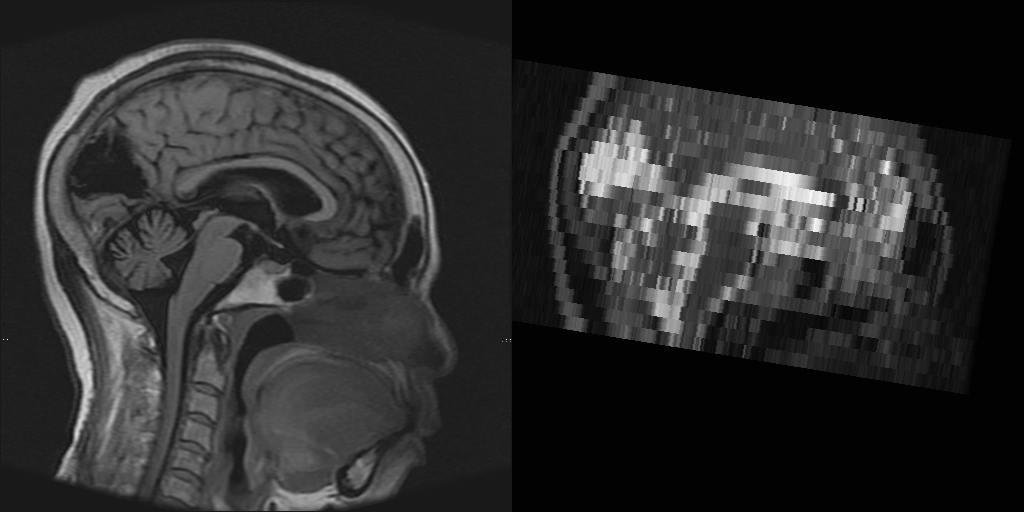
\includegraphics[width=\textwidth]{clinical_sag}

High resolution in-plane. Very thick slices.\par
Multiple image contrasts/orientations.\par
%More work needed for dealing with such data.
\end{frame}

\begin{frame}
\frametitle{Mining hospital data}
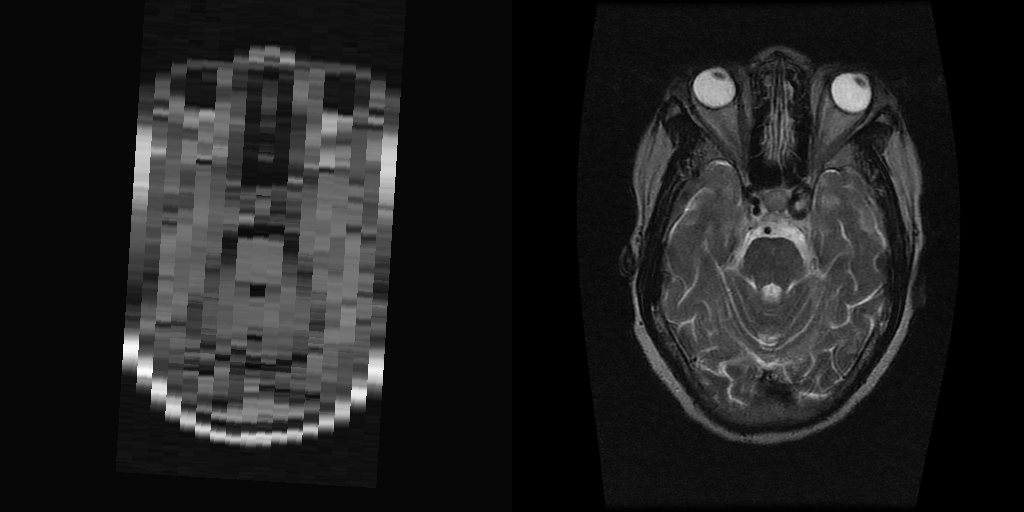
\includegraphics[width=\textwidth]{clinical_tra}

High resolution in-plane. Very thick slices.\par
Multiple image contrasts/orientations.\par
%More work needed for dealing with such data.
\end{frame}

\begin{frame}
\frametitle{Data sharing}
Increasing pressure from funding bodies to share data.
\begin{itemize}
\item Push for reproducible research.
\item Allows more discovery science.
\end{itemize}
... conflicts with personal privacy.

\vspace{0.25cm}
\begin{tiny}
\url{http://www.wellcome.ac.uk/About-us/Policy/Spotlight-issues/Data-sharing/}\par
\url{http://grants.nih.gov/grants/policy/data_sharing/}\par
%\url{http://www.mrc.ac.uk/research/research-policy-ethics/data-sharing/policy/}\par
\end{tiny}
\end{frame}

\begin{frame}
\frametitle{Bigger data}
{\bf UK Biobank Imaging} UK Biobank is a \emph{long-term prospective epidemiological study} that has already collected genetics, blood samples, lifestyle information and other data from a cohort of 500,000 subjects, to be followed clinically over coming decades.
The UK Biobank Imaging Extension, which aims to bring back \emph{100,000 of the cohort for multimodal neuroimaging} and cardiac MRI (amongst other measures), has just been given the go-ahead.
This will be by far the largest neuro/cardiac imaging study carried out to date, and will add very rich phenotyping to the overall Biobank project.
%Funded primarily by the MRC and Wellcome Trust, the initial phase will involve imaging several thousand subjects in a new, dedicated imaging centre, which, if shown to be successful, would expand into the full £36m imaging project, with two further dedicated imaging centres setup at other sites across the UK.
%Major input is coming from researchers at Oxford, Imperial, Southampton, Queen Mary College, Newcastle and Aberdeen; Prof Sir Rory Collins (CTSU, Oxford) is the overall UK Biobank PI, and Prof Paul Matthews (Imperial/GSK) is Chair of the Imaging Working Group.
%FMRIB (Smith, Miller), along with Matthews, is leading the neuroimaging - determining the imaging hardware setup, imaging protocols and post-processing pipeline, in consultation with the wider imaging community.
\end{frame}

